
%%%%%%%%%%%%%%%%%%%%%%%%%%%%%%%%%%%%%%%%%%%%%%%%%%%%%%%%%%%%%%%%%%%%%%%%%%%%%%%%%%
\begin{frame}[fragile]\frametitle{}

\begin{center}
{\Large Machine Learning (quick recap)}
\end{center}
\end{frame}


%%%%%%%%%%%%%%%%%%%%%%%%%%%%%%%%%%%%%%%%%%%%%%%%%%%%%%%%%%%%%%%%%%%%%%%%%%%%%%%%%%
\begin{frame}[fragile]\frametitle{Broad Categories of Machine Learning}
\adjustbox{valign=t}{
\begin{minipage}{0.45\linewidth}
Classification
\begin{itemize}
\item  Supervised ML
\item  Requires pre-labeled 
corpus of documents
\item  Sentiment Analysis
\item  Models: Naive Bayes, Maximum Entropy
\end{itemize}
\end{minipage}
}
\hfill
\adjustbox{valign=t}{
\begin{minipage}{0.4\linewidth}
Clustering
\begin{itemize}
\item Unsupervised ML
\item Groups similar 
documents together.
\item Topic Modeling
\item Models: LDA, NNMF
\end{itemize}

\end{minipage}
}

\end{frame}

%%%%%%%%%%%%%%%%%%%%%%%%%%%%%%%%%%%%%%%%%%%%%%%%%%%%%%%%%%%%%%%%%%%%%%%%%%%%%%%%%%
\begin{frame}[fragile]\frametitle{Supervised learning}
  \begin{itemize}
    \item Dataset consisting of labeled examples
    \item Each example has one or several attributes and a dependent variable (label, output, response, predicted variable)
    \item After building, selection and assessing the model on the labeled data, 
it is used to find labels for new data
  \end{itemize}
\end{frame}

%%%%%%%%%%%%%%%%%%%%%%%%%%%%%%%%%%%%%%%%%%%%%%%%%%%%%%%%%%%%%%%%%%%%%%%%%%%%%%%%%%
\begin{frame}[fragile]\frametitle{Supervised learning}
  \begin{itemize}
    \item Dataset is usually split into three parts : A rule is 50-25-25
    \item Training set
      \begin{itemize}
    \item Used to build models
    \item Compute the basic parameters of the model
      \end{itemize}
    \item Holdout/validation set
      \begin{itemize}
    \item Used to find out the best model and adjust some parameters of the model (usually, in order to minimize some error)
    \item Also called model selection
      \end{itemize}
    \item Test set
    \item Used to assess the final model on new data, after model building and selection
  \end{itemize}
\end{frame}

%%%%%%%%%%%%%%%%%%%%%%%%%%%%%%%%%%%%%%%%%%%%%%%%%%%%%%%%%%%%%%%%%%%%%%%%%%%%%%%%%%
\begin{frame}[fragile]\frametitle{Regression}
Supervised learning when the output variable is continuous 
\begin{center}
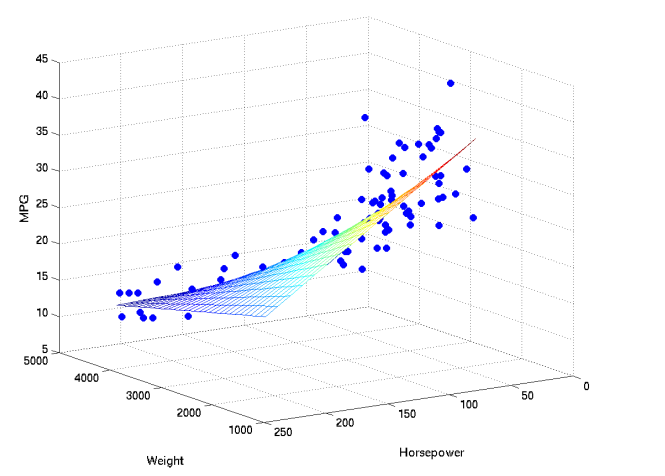
\includegraphics[width=0.8\linewidth,keepaspectratio]{regr}
\end{center}
\end{frame}

%%%%%%%%%%%%%%%%%%%%%%%%%%%%%%%%%%%%%%%%%%%%%%%%%%%%%%%%%%%%%%%%%%%%%%%%%%%%%%%%%%
\begin{frame}[fragile]\frametitle{Classification}
Supervised learning when the output variable is discrete (classes)
\begin{center}
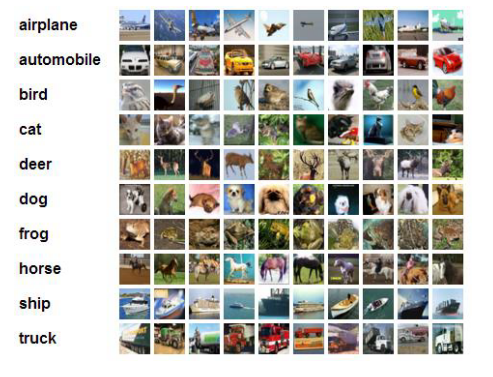
\includegraphics[width=0.8\linewidth,keepaspectratio]{class}
\end{center}
\end{frame}

%%%%%%%%%%%%%%%%%%%%%%%%%%%%%%%%%%%%%%%%%%%%%%%%%%%%%%%%%%%%%%%%%%%%%%%%%%%%%%%%%%
\begin{frame}[fragile]\frametitle{Classification Pipeline}
\begin{center}
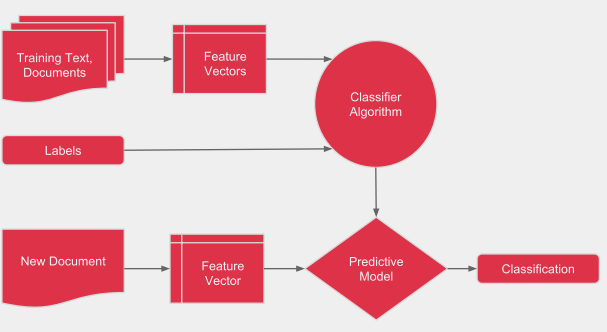
\includegraphics[width=\linewidth,keepaspectratio]{classpipe}
\end{center}
\end{frame}



%%%%%%%%%%%%%%%%%%%%%%%%%%%%%%%%%%%%%%%%%%%%%%%%%%%%%%%%%%%%%%%%%%%%%%%%%%%%%%%%%%
\begin{frame}[fragile]\frametitle{Unsupervised learning}
  \begin{itemize}
    \item  For an unlabeled dataset, infer properties (find ``hidden'' structure) about the distribution of the objects in the dataset 
    \item  Without any help related to correct answers

    \item Generally, much more data than for supervised learning
        \item There are several techniques that can be applied
      \begin{itemize}
    \item Clustering (cluster analysis)
    \item Dimensionality reduction (visualization of data)
    \item Association rules, frequent itemsets
      \end{itemize}

  \end{itemize}
\end{frame}

%%%%%%%%%%%%%%%%%%%%%%%%%%%%%%%%%%%%%%%%%%%%%%%%%%%%%%%%%%%%%%%%%%%%%%%%%%%%%%%%%%
\begin{frame}[fragile]\frametitle{Topic Modeling Pipeline}
\begin{center}
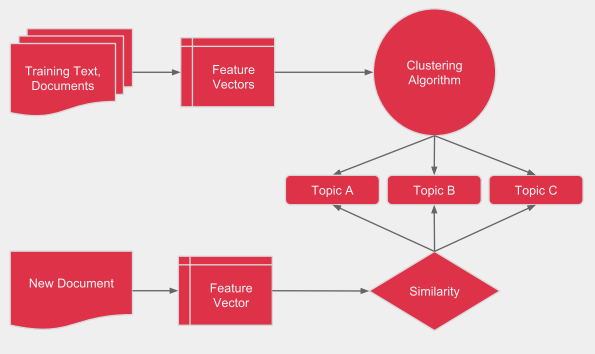
\includegraphics[width=\linewidth,keepaspectratio]{topicpipe}
\end{center}
\end{frame}


%%%%%%%%%%%%%%%%%%%%%%%%%%%%%%%%%%%%%%%%%%%%%%%%%%%%%%%%%%%%%%%%%%%%%%%%%%%%%%%%%%
\begin{frame}[fragile]\frametitle{Clustering}
  \begin{itemize}
    \item  Partition dataset into clusters (groups) of objects such that the ones in the same cluster are more similar to each other than to objects in different clusters
    \item Similarity
      \begin{itemize}
    \item The most important notion when clustering
    \item ``Inverse of a distance''
      \end{itemize}
	\item Possible objective: approximate the modes of the input dataset distribution
  \end{itemize}
\end{frame}

%%%%%%%%%%%%%%%%%%%%%%%%%%%%%%%%%%%%%%%%%%%%%%%%%%%%%%%%%%%%%%%%%%%%%%%%%%%%%%%%%%
\begin{frame}[fragile]\frametitle{Dimensionality reduction}
  \begin{itemize}
    \item  Usually, unsupervised datasets are large both in number of examples  and in number of attributes (features)
    \item  Reduce the number of features in order to improve (human) readability and interpretation of data
    \item  Mainly linked to visualization
    \item  Also used for feature selection, data compression or denoising
  \end{itemize}
\end{frame}

%%%%%%%%%%%%%%%%%%%%%%%%%%%%%%%%%%%%%%%%%%%%%%%%%%%%%%%%%%%%%%%%%%%%%%%%%%%%%%%%%%
\begin{frame}[fragile]\frametitle{Performance measures - supervised}
  \begin{itemize}
    \item  Regression
      \begin{itemize}
    \item   Mean error, mean squared error (MSE), root MSE, etc.
  \end{itemize}
      \item  Classification
      \begin{itemize}
    \item  Accuracy
    \item  Precision / recall (possibly weighted)
    \item  F-measure
    \item  Confusion matrix
    \item  TP, TN, FP, FN
    \item  AUC / ROC
  \end{itemize}
  \end{itemize}
\end{frame}

%%%%%%%%%%%%%%%%%%%%%%%%%%%%%%%%%%%%%%%%%%%%%%%%%%%%%%%%%%%%%%%%%%%%%%%%%%%%%%%%%%
\begin{frame}[fragile]\frametitle{Metrics}
\begin{center}
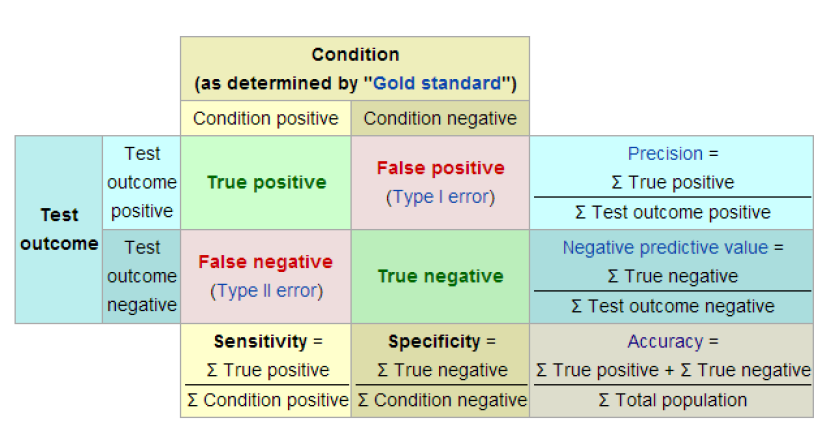
\includegraphics[width=\linewidth,keepaspectratio]{metrics}
\end{center}
\end{frame}

%%%%%%%%%%%%%%%%%%%%%%%%%%%%%%%%%%%%%%%%%%%%%%%%%%%%%%%%%%%%%%%%%%%%%%%%%%%%%%%%%%
\begin{frame}[fragile]\frametitle{Basic Notions of ML}
  \begin{itemize}
    \item  Overfitting
      \begin{itemize}
    \item   Low error on training data
    \item   High error on (unseen/new) test data
    \item   The model does not generalize well from the training data on unseen data
    \item   Possible causes:
    \item   Too few training examples
    \item   Model too complex (too many parameters)
  \end{itemize}
    \item  Underfitting
      \begin{itemize}
    \item    High error both on training and test data
    \item    Model is too simple to capture the information in the training data
  \end{itemize}
  \end{itemize}
\end{frame}

%%%%%%%%%%%%%%%%%%%%%%%%%%%%%%%%%%%%%%%%%%%%%%%%%%%%%%%%%%%%%%%%%%%%%%%%%%%%%%%%%%
\begin{frame}[fragile]\frametitle{ML conclusions}
  \begin{itemize}
    \item  Feature extraction is important in ML
    \item Which are the best features?
    \item Syntactic and context analysis are the most important
    \item Semantic analysis is slow but increases detection by 10\%
    \item Using features related to users would further improve our results
    % \item Not always! Maybe another discussion on this
      \end{itemize}
\end{frame}


%%%%%%%%%%%%%%%%%%%%%%%%%%%%%%%%%%%%%%%%%%%%%%%%%%%%%%%%%%%%%%%%%%%%%%%%%%%%%%%%%%
\begin{frame}[fragile]\frametitle{}

\begin{center}
{\Large Machine Learning in NLP}
\end{center}
\end{frame}

% %%%%%%%%%%%%%%%%%%%%%%%%%%%%%%%%%%%%%%%%%%%%%%%%%%%%%%%%%%%%%%%%%%%%%%%%%%%%%%%%%%
% \begin{frame}[fragile] \frametitle{Why machine learning?}

  % \begin{itemize}
    % \item `` Simply put, machine learning is the part of artificial intelligence that actually works''
    % \item Most popular course on Coursera
    % \item Meaning practical: ML results are nice and easy to show to others
    % \item Meaning well-paid/in demand: companies are increasing demand for ML specialists
    % \item Large volumes of data, corpora, etc
  % \end{itemize}
% \end{frame}

%%%%%%%%%%%%%%%%%%%%%%%%%%%%%%%%%%%%%%%%%%%%%%%%%%%%%%%%%%%%%%%%%%%%%%%%%%%%%%%%%%
\begin{frame}[fragile]
  \frametitle{Most important, for ML: Features}
\begin{lstlisting}
>>> text = "Seven-time Formula One champion Michael Schumacher took on the Shanghai circuit Saturday in qualifying for the first Chinese Grand Prix." 
>>> label = ``sport'' 
\end{lstlisting}
\begin{itemize}
\item Here the classification takes as input the whole string
\item What's the problem with  that?
\item What are the features that could be useful for this example?
\end{itemize}
\end{frame}

%%%%%%%%%%%%%%%%%%%%%%%%%%%%%%%%%%%%%%%%%%%%%%%%%%%%%%%%%%%%%%%%%%%%%%%%%%%%%%%%%%
\begin{frame}[fragile]
  \frametitle{Feature terminology}
\begin{itemize}
\item Feature: An aspect of the text  that is relevant to the task
\item Feature value: the realization of the feature in the text
\item Some typical features
\begin{itemize}
\item Words present in text : Kerry, Schumacher, China\ldots 
\item Frequency of word: Kerry(10), Schumacher(1)\ldots
\item Are there dates? Yes/no
\item Capitalization (is word capitalized?)
\item Are there PERSONS? Yes/no
\item Are there ORGANIZATIONS? Yes/no
\item WordNet: Holonyms (China is part of Asia), Synonyms(China, People's Republic of China, mainland China)
\item Chunks, parse trees, POS
\end{itemize}
\end{itemize}
\end{frame}

%%%%%%%%%%%%%%%%%%%%%%%%%%%%%%%%%%%%%%%%%%%%%%%%%%%%%%%%%%%%%%%%%%%%%%%%%%%%%%%%%%
\begin{frame}[fragile]\frametitle{Document Features}
Features describe instances in a 
way that machines can learn on by 
putting them into feature space.

\adjustbox{valign=t}{
\begin{minipage}{0.45\linewidth}
\begin{itemize}
\item Document level features
\begin{itemize}
\item  Metadata: title, author
\item Paragraphs
\item Sentence construction 
\end{itemize}
\item Word level features
\begin{itemize}
\item  Vocabulary 
\item  Form (capitalization)
\item  Frequency  
\end{itemize}
\end{itemize}
\end{minipage}
}
\hfill
\adjustbox{valign=t}{
\begin{minipage}{0.45\linewidth}
\begin{center}
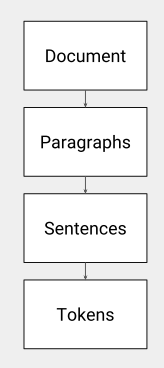
\includegraphics[width=0.6\linewidth,keepaspectratio]{docpipe}
\end{center}
\end{minipage}
}
%\begin{lstlisting}
%# Creates a graph.
%with tf.device('/gpu:2'):
%	a = tf.constant([1.0], name='a')
%	b = tf.constant([1.0], name='b')
%	c = tf.matmul(a, b)
%\end{lstlisting}
\end{frame}

%%%%%%%%%%%%%%%%%%%%%%%%%%%%%%%%%%%%%%%%%%%%%%%%%%%%%%%%%%%%%%%%%%%%%%%%%%%%%%%%%%
\begin{frame}[fragile]\frametitle{Vector Encoding}
ML needs data (text in this case) in Vector/Numeric form.
\begin{itemize}
\item  Basic representation of documents: a vector whose length is equal to the vocabulary of the entire corpus. 
\item  Word positions in the vector are based on lexicographic order.
\end{itemize}
\begin{center}
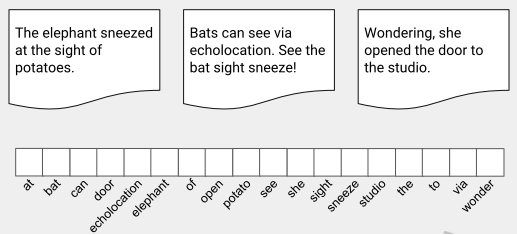
\includegraphics[width=\linewidth,keepaspectratio]{vect}
\end{center}
\end{frame}

%%%%%%%%%%%%%%%%%%%%%%%%%%%%%%%%%%%%%%%%%%%%%%%%%%%%%%%%%%%%%%%%%%%%%%%%%%%%%%%%%%
\begin{frame}[fragile]\frametitle{Bag of Words: Token Frequency}
\begin{itemize}
\item  One of the simplest models: compute the frequency of words in 
the document and use those numbers as the vector encoding.
\end{itemize}
\begin{center}
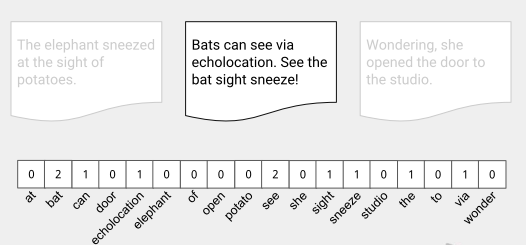
\includegraphics[width=\linewidth,keepaspectratio]{bow}
\end{center}
\end{frame}

%%%%%%%%%%%%%%%%%%%%%%%%%%%%%%%%%%%%%%%%%%%%%%%%%%%%%%%%%%%%%%%%%%%%%%%%%%%%%%%%%%
\begin{frame}[fragile]\frametitle{One Hot Encoding}
\begin{itemize}
\item   The feature vector encodes the vocabulary of the document. 
\item  All words are equally distant, so must reduce word forms. 
\item  Usually used for artificial neural network models.
\end{itemize}
\begin{center}
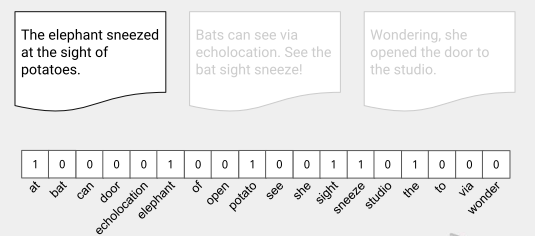
\includegraphics[width=\linewidth,keepaspectratio]{onehot}
\end{center}
\end{frame}

%%%%%%%%%%%%%%%%%%%%%%%%%%%%%%%%%%%%%%%%%%%%%%%%%%%%%%%%%%%%%%%%%%%%%%%%%%%%%%%%%%
\begin{frame}[fragile]\frametitle{TF-IDF Encoding}
\begin{itemize}
\item   Highlight terms that are very relevant to a document relative to 
the rest of the corpus by computing the term frequency times 
the inverse document frequency of the term. 
\end{itemize}
\begin{center}
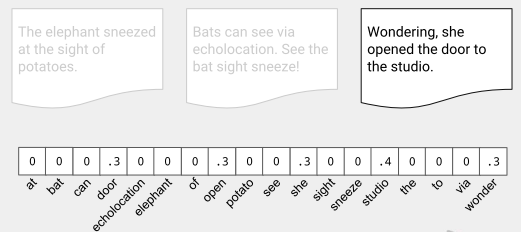
\includegraphics[width=\linewidth,keepaspectratio]{tfidf}
\end{center}
\end{frame}


%%%%%%%%%%%%%%%%%%%%%%%%%%%%%%%%%%%%%%%%%%%%%%%%%%%%%%%%%%%%%%%%%%%%%%%%%%%%%%%%%%
\begin{frame}[fragile]\frametitle{Pros and Cons of Vector Encoding}
\adjustbox{valign=t}{
\begin{minipage}{0.45\linewidth}
Pros
\begin{itemize}
\item  Machine learning requires 
a vector anyway. 
\item Can embed complex 
representations like TF-IDF 
into the vector form. 
\item Drives towards token-
concept mapping without 
rules.
\end{itemize}
\end{minipage}
}
\hfill
\adjustbox{valign=t}{
\begin{minipage}{0.4\linewidth}
Cons
\begin{itemize}
\item The vectors have lots of columns (high dimension)
\item Word order, grammar, and 
other structural features 
are natively lost. 
\item Difficult to add knowledge 
to learning process. 
\end{itemize}

\end{minipage}
}

\end{frame}


%%%%%%%%%%%%%%%%%%%%%%%%%%%%%%%%%%%%%%%%%%%%%%%%%%%%%%%%%%%%%%%%%%%%%%%%%%%%%%%%%%%
%\begin{frame}[fragile]\frametitle{Vectorization in Machine learning}
%  \begin{center}
%In the end, much of the work for 
%language aware applications 
%comes from domain specific 
%feature analysis; not just simple 
%vectorization. 
%  \end{center}
%\end{frame}

%%%%%%%%%%%%%%%%%%%%%%%%%%%%%%%%%%%%%%%%%%%%%%%%%%%%%%%%%%%%%%%%%%%%%%%%%%%%%%%%%%
\begin{frame}[fragile]
  \frametitle{Feature selection}
\begin{itemize}
\item Selecting relevant features and deciding how to encode them for a learning method can have an enormous impact on the learning method's ability to extract a good model
\item How do we choose the ``right'' features?
\item Typically, feature extractors are built through a process of trial-and-error, guided by intuitions about what information is relevant to the problem. 
\item But there are also more ``principled'' way of features selection 

\end{itemize}
\end{frame}

%%%%%%%%%%%%%%%%%%%%%%%%%%%%%%%%%%%%%%%%%%%%%%%%%%%%%%%%%%%%%%%%%%%%%%%%%%%%%%%%%%
\begin{frame}[fragile]
  \frametitle{Feature selection}
\begin{itemize}
\item There are usually limits to the number of features that you should use with a given learning algorithm
\item If you provide too many features, then the algorithm will have a higher chance of relying on idiosyncrasies of your training data that don't generalize well to new examples. 
\item This problem is known as overfitting, and can be especially problematic when working with small training sets. 
\end{itemize}
\end{frame}

%%%%%%%%%%%%%%%%%%%%%%%%%%%%%%%%%%%%%%%%%%%%%%%%%%%%%%%%%%%%%%%%%%%%%%%%%%%%%%%%%%
\begin{frame}[fragile]
  \frametitle{Feature selection}
\begin{itemize}
\item Once an initial set of features has been chosen, a very productive method for refining the feature set is error analysis. First, we select a development set, containing the corpus data for creating the model. This development set is then subdivided into the training set and the dev-test set.
\item The training set is used to train the model, and the dev-test set is used to perform error analysis. 
Look at errors, change features or model
\item The test set serves in our final evaluation of the system
\end{itemize}
\end{frame}

%%%%%%%%%%%%%%%%%%%%%%%%%%%%%%%%%%%%%%%%%%%%%%%%%%%%%%%%%%%%%%%%%%%%%%%%%%%%%%%%%%
\begin{frame}[fragile]\frametitle{Features}
\begin{center}
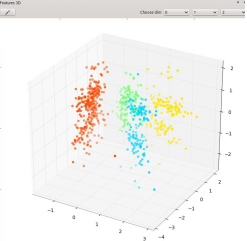
\includegraphics[width=0.4\linewidth,keepaspectratio]{feats}

\end{center}

Features describe instances in a 
way that machines can learn on by 
putting them into feature space.
\end{frame}


%%%%%%%%%%%%%%%%%%%%%%%%%%%%%%%%%%%%%%%%%%%%%%%%%%%%%%%%%%%%%%%%%%%%%%%%%%%%%%%%%%%
%\begin{frame}[fragile]\frametitle{Example: Finding Vandalism on Wikipedia }
%  \begin{itemize}
%    \item  Vandalism = editing in a malicious manner that is intentionally disruptive
%    \item Dataset used at PAN 2011
%          \begin{itemize}
%    \item Real articles extracted from Wikipedia in 2009 and 2010
%    \item Training data: 32,000 edits
%    \item Test data: 130,000 edits
%      \end{itemize}
%    \item An edit consists of:
%          \begin{itemize}
%    \item the old and new content of the article
%    \item author information
%    \item revision comment and timestamp
%      \end{itemize}
%    \item We chose to use only the actual text in the revision (no author and timestamp information) to predict vandalism
%      \end{itemize}
%\end{frame}
%
%%%%%%%%%%%%%%%%%%%%%%%%%%%%%%%%%%%%%%%%%%%%%%%%%%%%%%%%%%%%%%%%%%%%%%%%%%%%%%%%%%%
%\begin{frame}[fragile]\frametitle{Features}
%\begin{center}
%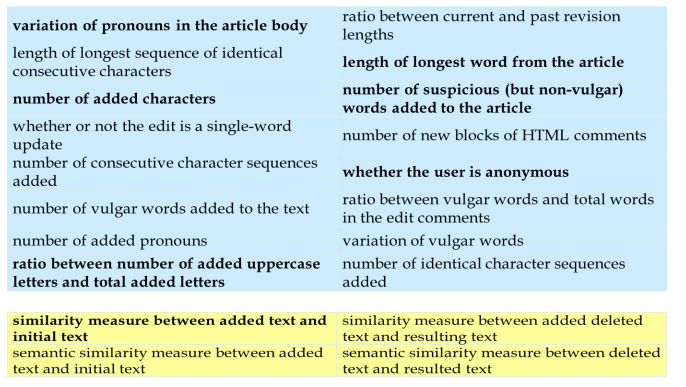
\includegraphics[width=\linewidth,keepaspectratio]{features}
%\end{center}
%\end{frame}

%%%%%%%%%%%%%%%%%%%%%%%%%%%%%%%%%%%%%%%%%%%%%%%%%%%%%%%%%%%%%%%%%%%%%%%%%%%%%%%%%%
\begin{frame}[fragile]\frametitle{Using several classifiers}
\begin{center}
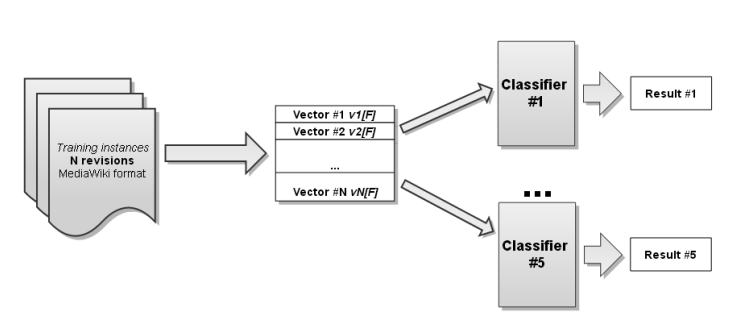
\includegraphics[width=\linewidth,keepaspectratio]{sevclass}
\end{center}
\end{frame}

%%%%%%%%%%%%%%%%%%%%%%%%%%%%%%%%%%%%%%%%%%%%%%%%%%%%%%%%%%%%%%%%%%%%%%%%%%%%%%%%%%
\begin{frame}[fragile]\frametitle{Cross-validation results}
\begin{center}
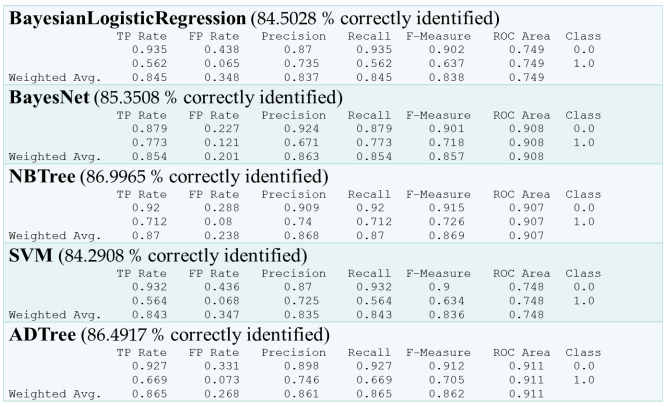
\includegraphics[width=\linewidth,keepaspectratio]{crossval}
\end{center}
\end{frame}





%%%%%%%%%%%%%%%%%%%%%%%%%%%%%%%%%%%%%%%%%%%%%%%%%%%%%%%%%%%%%%%%%%%%%%%%%%%%%%%%%%
\begin{frame}[fragile]\frametitle{ML + NLP: Conclusions}
  \begin{itemize}
      \item A meta-classifier sometimes improves the results of several individual classifiers

    \item Lots of interesting ML+NLP tasks and data available
	
    \item Do you have access to new and interesting data in your business?
    % \item Several programming alternatives, easy to use
    % \item Understand the basics
    % \item Enhance your Maths (statistics) skills for a better ML experience
    % \item Hands-on experience and communities of practice
    % \item www.kaggle.com (and other similar initiatives)
          \end{itemize}
\end{frame}





